\newpage
\section{Introduction} 

The ability to adapt in minutes is a defining characteristic of human intelligence and an important milestone on the path towards general intelligence. Given any level of bounded rationality, there will be a space of tasks in which it is impossible for agents to succeed by just generalising their policy zero-shot, but where progress is possible if the agent is capable of very fast in-context learning from feedback. To be useful in the real world, and in interaction with humans, our artificial agents should be capable of fast and flexible adaptation given only a few interactions, and should continue to adapt as more data becomes available. Operationalising this notion of adaptation, we seek to train an agent that, given few episodes in an unseen environment at test time, can accomplish a task that requires trial-and-error exploration and can subsequently refine its solution towards optimal behaviour.

Meta-RL has been shown to be effective for fast in-context adaptation (e.g. \citet{yu2020learning, zintgraf2022fast}). However, meta-RL has had limited success in settings where the reward is sparse and the task space is vast and diverse \citep{yang2019single}. Outside RL, \emph{foundation models} in semi-supervised learning have generated significant interest \citep{DBLP:journals/corr/abs-2108-07258} due to their ability to adapt in few shots from demonstrations across a broad range of tasks. These models are designed to provide a strong foundation of general knowledge and skills that can be built upon and adapted to new situations via fine-tuning or prompting with demonstrations~\citep{brown2020gpt3}. Crucial to this success has been attention-based memory architectures like Transformers \citep{vaswani2017attention}, which show power-law scaling in performance with the number of parameters \citep{https://doi.org/10.48550/arxiv.2207.10551}.


\begin{figure}[htb]
    \centering
    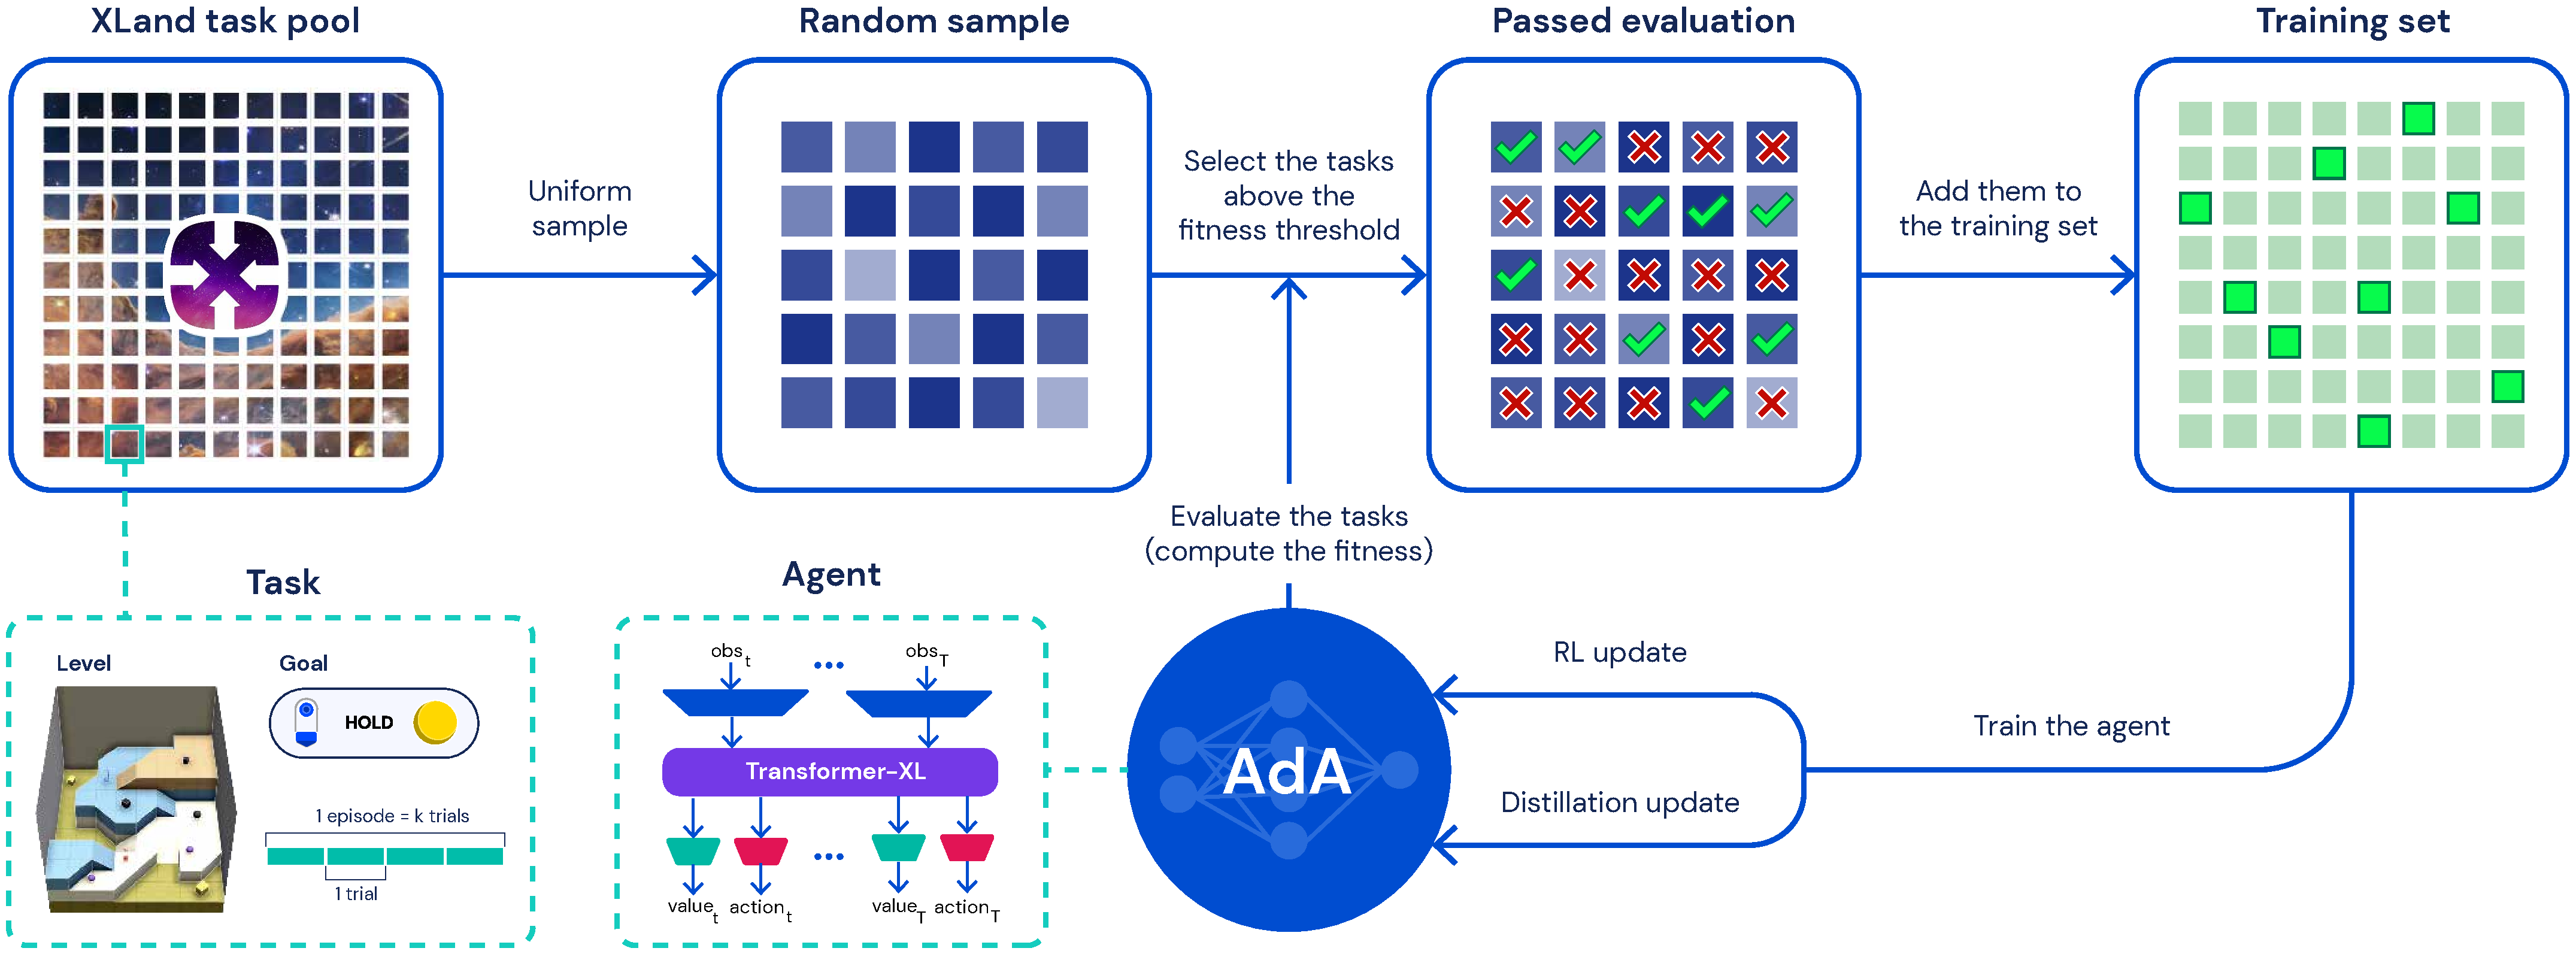
\includegraphics[width=\linewidth]{figures/ada_paper_diagrams_overview.pdf}
    \caption{
        \textbf{Training our Adaptive Agent (AdA).} We train a large Transformer model with meta-RL in XLand. During training, tasks are uniformly sampled, and subsequently filtered to produce an ever-changing training pool of tasks at the frontier of the agent's capabilities. After training on these tasks, the agent is capable of adapting to unseen hand-authored tasks as effectively and efficiently as humans.}
    \label{fig:method_overview}
\end{figure}


In this work, we pave the way for training an RL foundation model; that is, an agent that has been pre-trained on a vast task distribution and that, at test time, can adapt few-shot to a broad range of downstream tasks. We introduce \emph{Adaptive Agent} (AdA), an agent capable of human-timescale adaptation in a vast open-ended task space with sparse rewards. AdA does not require any prompts \citep{reed2022a}, fine-tuning \citep{lee2022multigame} or access to offline datasets \citep{laskin2022algorithmdistillation, reed2022a}. Instead, AdA exhibits hypothesis-driven exploratory behaviour, using information gained on-the-fly to refine its policy and to achieve close to optimal performance. AdA acquires knowledge efficiently, adapting in minutes on challenging held-out sparse-reward tasks in a partially-observable 3D environment with a first-person pixel observation. A human study confirms that the timescale of AdA's adaptation is comparable to that of trained human players. AdA's adaptation behaviour in a representative held-out task can be seen in Figure \ref{fig:intro-pyramid-in-a-haystack-explained}. AdA can also achieve improved performance through zero-shot prompting with first-person demonstrations, analogously to foundation models in the language domain.

We use Transformers as an architectural choice to scale in-context fast adaptation via model-based RL${^2}$ \citep{duan2017rl, wang2016learning, melo2022transformers}. Foundation models typically require large, diverse datasets to achieve their generality \citep{8237359, mahajan2018, brown2020gpt3, 9880094, schuhmann2022laionb}. To make this possible in an RL setting, where agents collect their own data, we extend the recent XLand environment \citep{xland}, producing a vast open-ended world with over $10^{40}$ possible tasks. These tasks require a range of different online adaptation capabilities, including experimentation, navigation, coordination, division of labour and coping with irreversibility. Given the wide range of possible tasks, we make use of adaptive auto-curricula, which prioritise tasks at the frontier of an agent's capabilities~\citep{xland, jiang2021robustplr}. Finally, we make use of distillation \citep{schmitt2018kickstarting}, which enables scaling to models with over 500M parameters, to the best of our knowledge the largest model trained from scratch with RL at the time of publication \citep{https://doi.org/10.48550/arxiv.2102.07920}. A high level overview of our method is shown in Figure~\ref{fig:method_overview}. 

Our main contributions are as follows:

\begin{itemize}
    \item We introduce AdA, an agent capable of human-timescale adaptation in a wide range of challenging tasks.
    \item We train AdA using meta-RL at scale in an open-ended task space with an automated curriculum.
    \item We show that adaptation is
    influenced by memory architecture, curriculum, and the size and complexity of the training task distribution.
    \item We produce scaling laws in both model size and memory, and demonstrate that AdA improves its performance with zero-shot first-person prompting. 
\end{itemize}